  \ac{RIA} ist kein Standard, sondern ein synonym für Applikationen, welche
  eine ``reichhaltige'' Benutzeroberfläche bieten und eine Verbindung mit dem
  Internet haben. Siehe \cite{RichInternetApplication}.
  
  \section{Grundlagen}
  
  Der Begriff \ac{RIA} ist mit der Entwicklung des Internets entstanden und
  wird heute oft verwendet. Für viele Leute ist \ac{RIA} ein synonmy für
  Webanwendungen, welche mit \ac{Ajax} realisiert werden. \ac{Ajax} bietet die
  Möglichkeit eine ``reichhaltige'' Benutzeroberfläche zu entwickeln, so wie
  man sich das von klassischen Desktopanwendungen gewöhnt ist. Die Grenze
  zwischen der klassischen Webanwendung und einer Desktopapplikation scheint
  damit zu verschwinden. Genauer betrachtet steht eine \ac{RIA} im
  Technologiespektrum aber zwischen dem Rich Client und dem Thin Client, siehe
  Grafik \ref{img:webanwendungen}.
  
  \begin{figure}[h]
    \begin{center}
      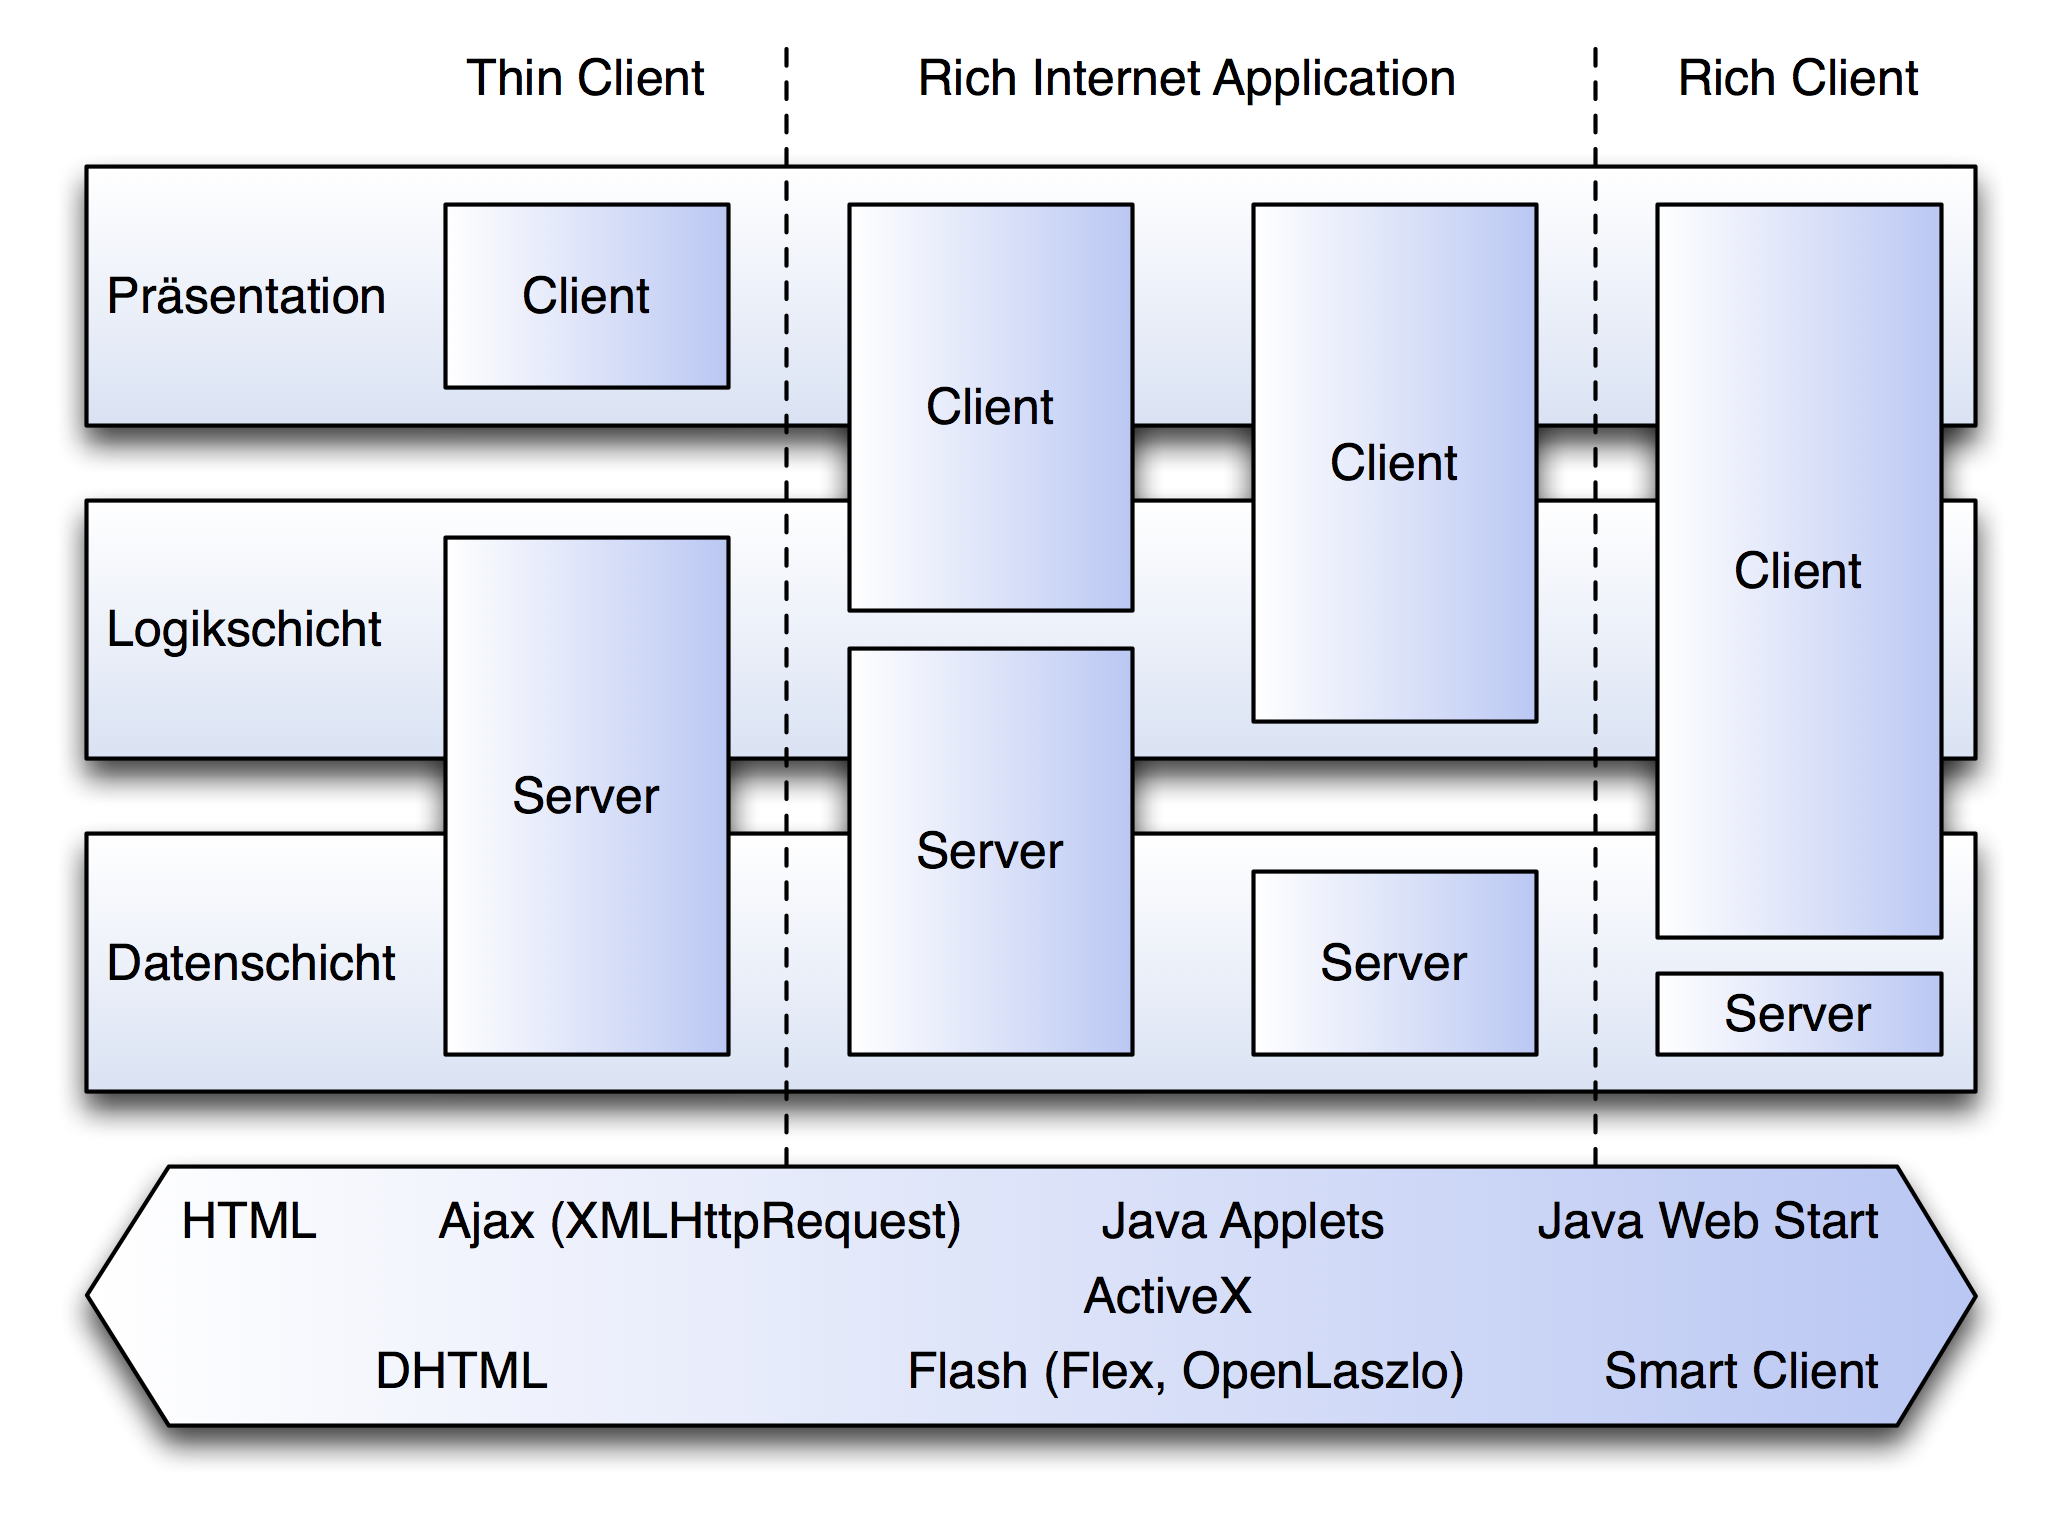
\includegraphics[width=0.7\textwidth]{./image/webanwendungen.png}
      \caption{Web Anwendungen (nach \cite{DiplomarbeitStephanSchuster} S. 6f.
      und \cite{WebApplicationSolutions} S. 5)}
      \label{img:webanwendungen}
    \end{center}
  \end{figure}
  
  Rich Client steht für kompilierte Desktopapplikationen und Thin Client für
  Webapplikationen welche im Webbrowser laufen, siehe
  \cite{WebApplicationSolutions} S. 4f. Da die Grenze zwischen \ac{RIA} und
  Thin Client nicht klar definiert ist, kommt ab und zu auch der Begriff von
  Thin Client zum Einsatz.
  
  \subsection{Browser orientiert}
  
  Browser orientierte \ac{RIA} kommen aus der evolution der Internettechnologie
  heraus, da sich deren Grundkonzepte in den letzten Jahren verändert haben. Um
  die Jahrtausenwende wurden klassische Webanwendung nach dem Prinzip von
  Request - Response aufgebaut. Der Benutzer konnte mit einer Interaktion einen
  Statuswechsel von einer Seite zur Nächsten auslösen, zum Beispiel durch das
  anklicken eines Links oder mit dem Versenden eines HTML-Formulars, siehe
  Grafik \ref{img:classicPageReload}. Dabei wurde immer der gesamte
  Seiteninhalt neu geladen, was zu längeren wartezeiten beim Laden der Seite
  und zu einem ungewohnten Anwendergefühl, im Vergleich zu Desktopanwengungen,
  geführt hat. Zudem werden immer alle Daten vom Server an den Browser
  übermittelt, welche für die Darstellung der Webanwendung von Nöten war, siehe
  \cite{AjaxInAction} S.44ff.
  
  \begin{figure}[h]
    \begin{center}
      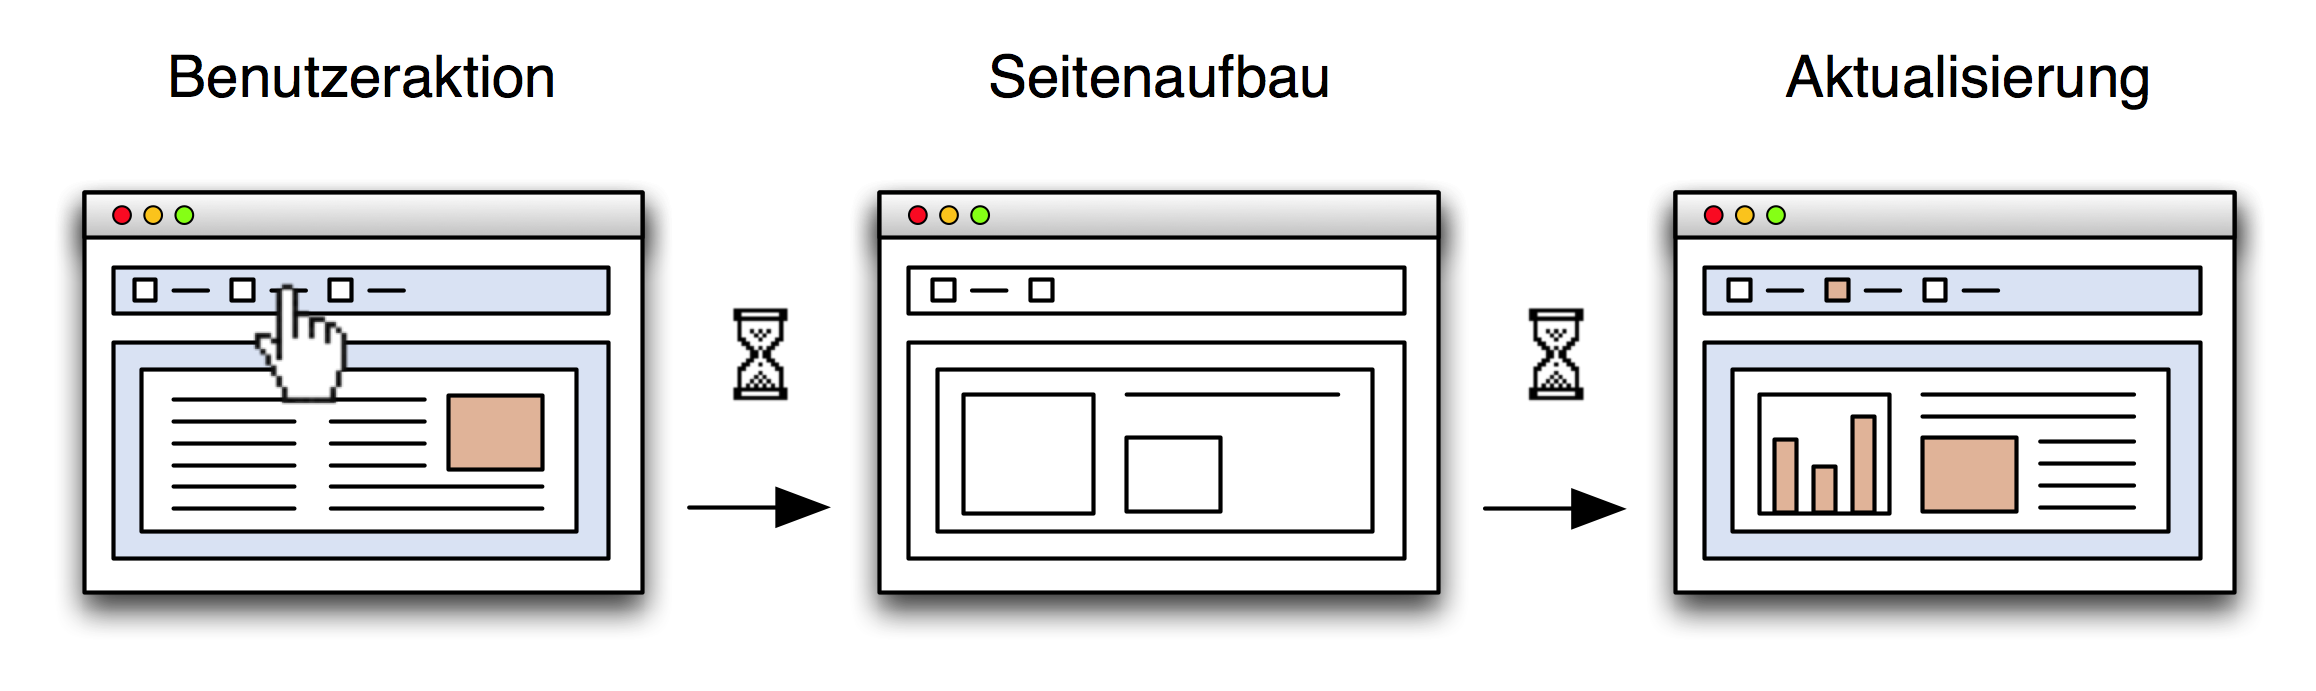
\includegraphics[width=0.95\textwidth]{./image/classicPageReload.png}
      \caption{Klassische Webanwendung aus der Usersicht (nach
      \cite{DiplomarbeitStephanSchuster} S. 10)}
      \label{img:classicPageReload}
    \end{center}
  \end{figure}
  
  In einem \ac{UML} Sequenzdiagramm sieht das wie folgt aus, siehe Grafik
  \ref{img:sequenzdiagrammClassicPageReload}.
  
  \begin{figure}[h]
    \begin{center}
      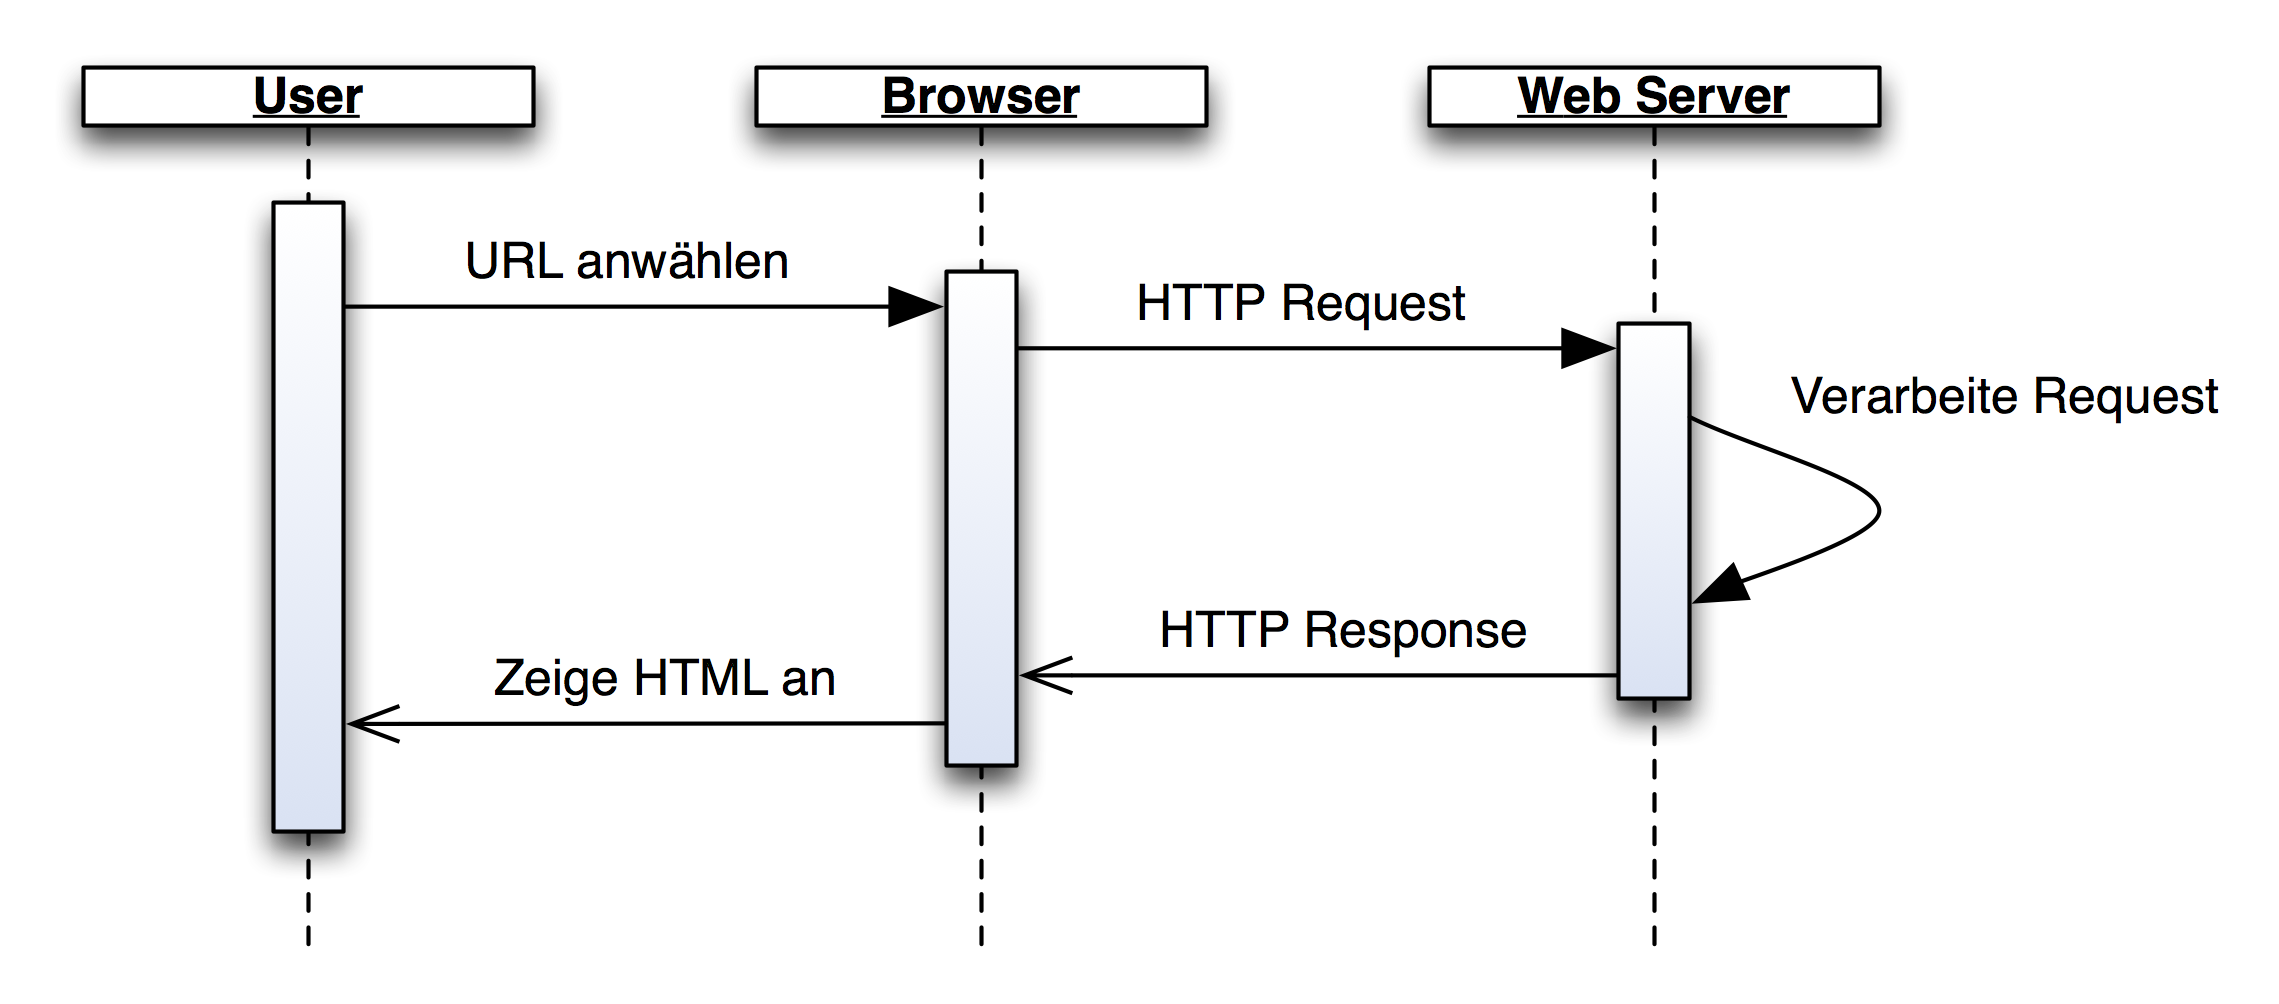
\includegraphics[width=0.7\textwidth]{./image/sequenzdiagrammClassicPageReload.png}
      \caption{HTTP Request als \ac{UML} Sequenzdiagramm (nach
      \cite{HttpBasics} S. 10)}
      \label{img:sequenzdiagrammClassicPageReload}
    \end{center}
  \end{figure}
  
  Mit dem Konzept von \ac{Ajax}, bei dem der Browser asynchron Daten vom Server
  nachladen kann, wurde die Möglichkeit geschaffen, Anwendungen zu entwickeln,
  welche sich in der Bedienung wie Desktopanwendungen anfühlen, siehe Grafik
  \ref{img:ajaxPageReload}. Das Prinzip funktioniert dadruch, dass eine
  zusätzliche Schicht zwischen dem Browser und Server eingerichtet wird. Diese
  Schicht, ich nenne sie hier Ajax-Engine, übernimmt die Kontrolle über die
  Datenkommunikation zum Server. Die Ajax-Engine bietet die Möglichkeit
  asynchron zur Clientinteraktion Daten vom Server anzufordern und bei Erhalt
  dynamisch in die bestehende Seite einzuflechten. Das Ergebnis ist, dass der
  Browser vom Server entkoppelt wird, wobei der Benutzer die Seite weiterhin
  verwenden kann, auch der Server im Hintergrund getätigte Interaktionen
  verarbeitet.
  
  \begin{figure}[h]
    \begin{center}
      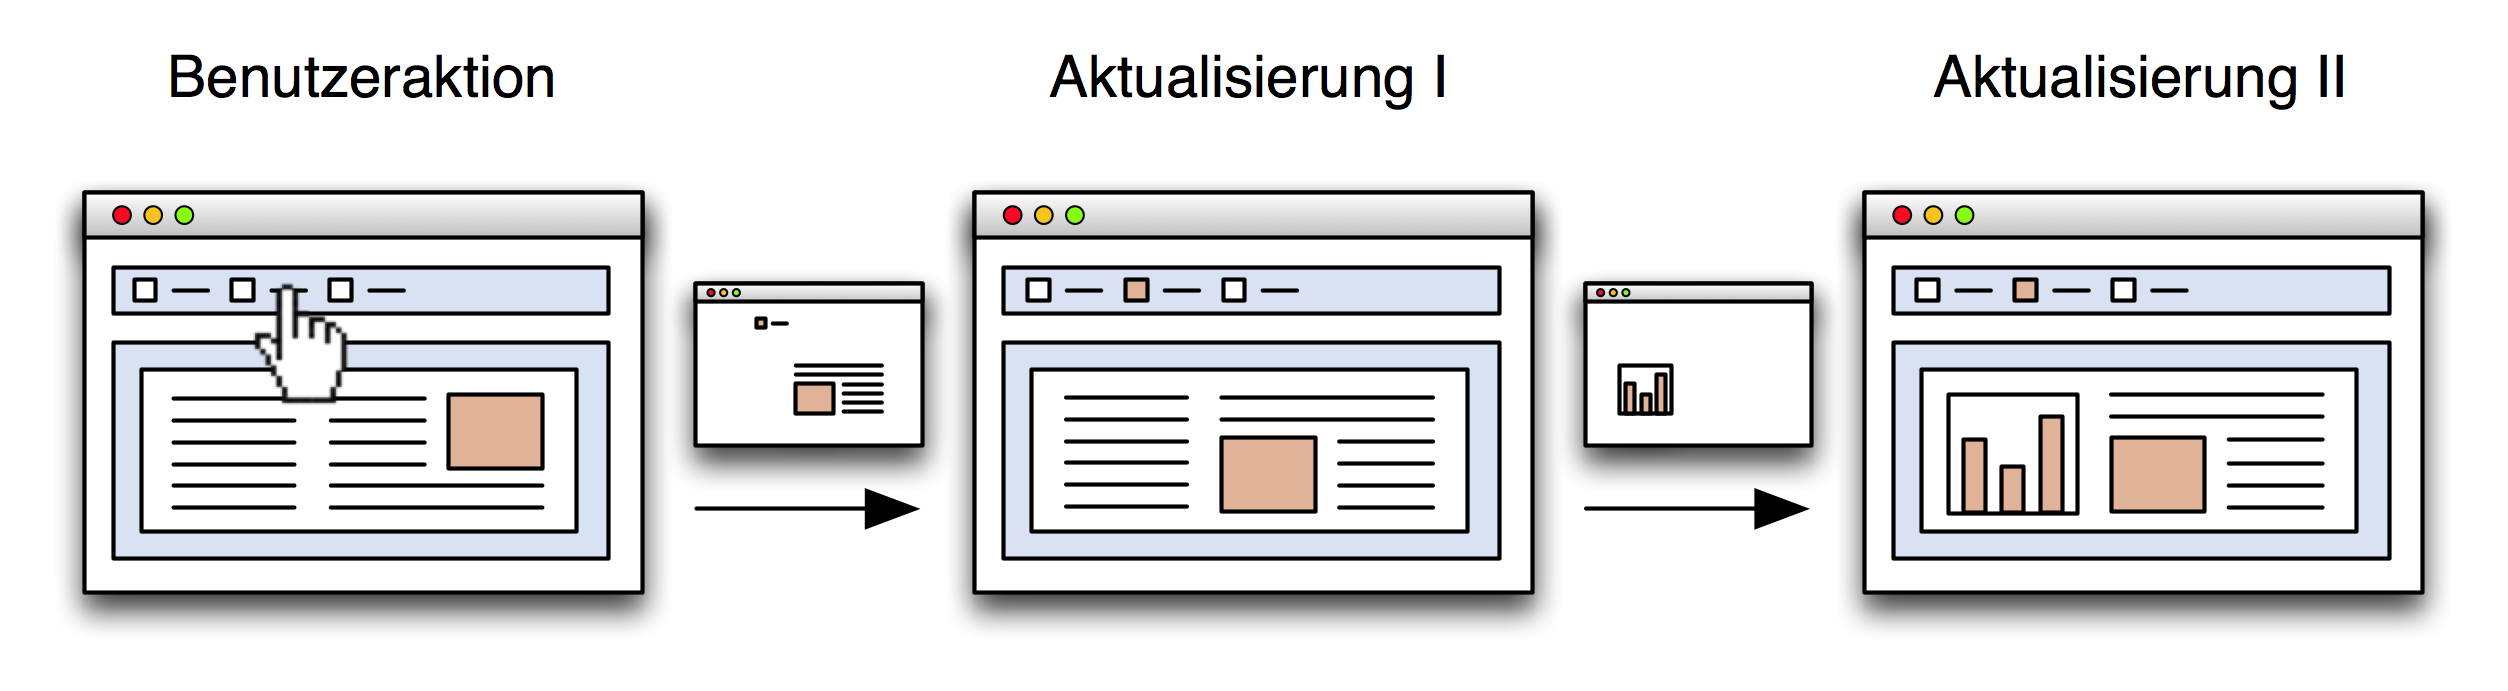
\includegraphics[width=0.7\textwidth]{./image/ajaxPageReload.png}
      \caption{Webanwendung mit Ajax aus der Usersicht (nach
      \cite{DiplomarbeitStephanSchuster} S.12)}
      \label{img:ajaxPageReload}
    \end{center}
  \end{figure}
  
  In einem \ac{UML} Sequenzdiagramm sieht das wie folgt aus, siehe Grafik
  \ref{img:sequenzdiagrammAjaxPageReload}.
  
  \begin{figure}[h]
    \begin{center}
      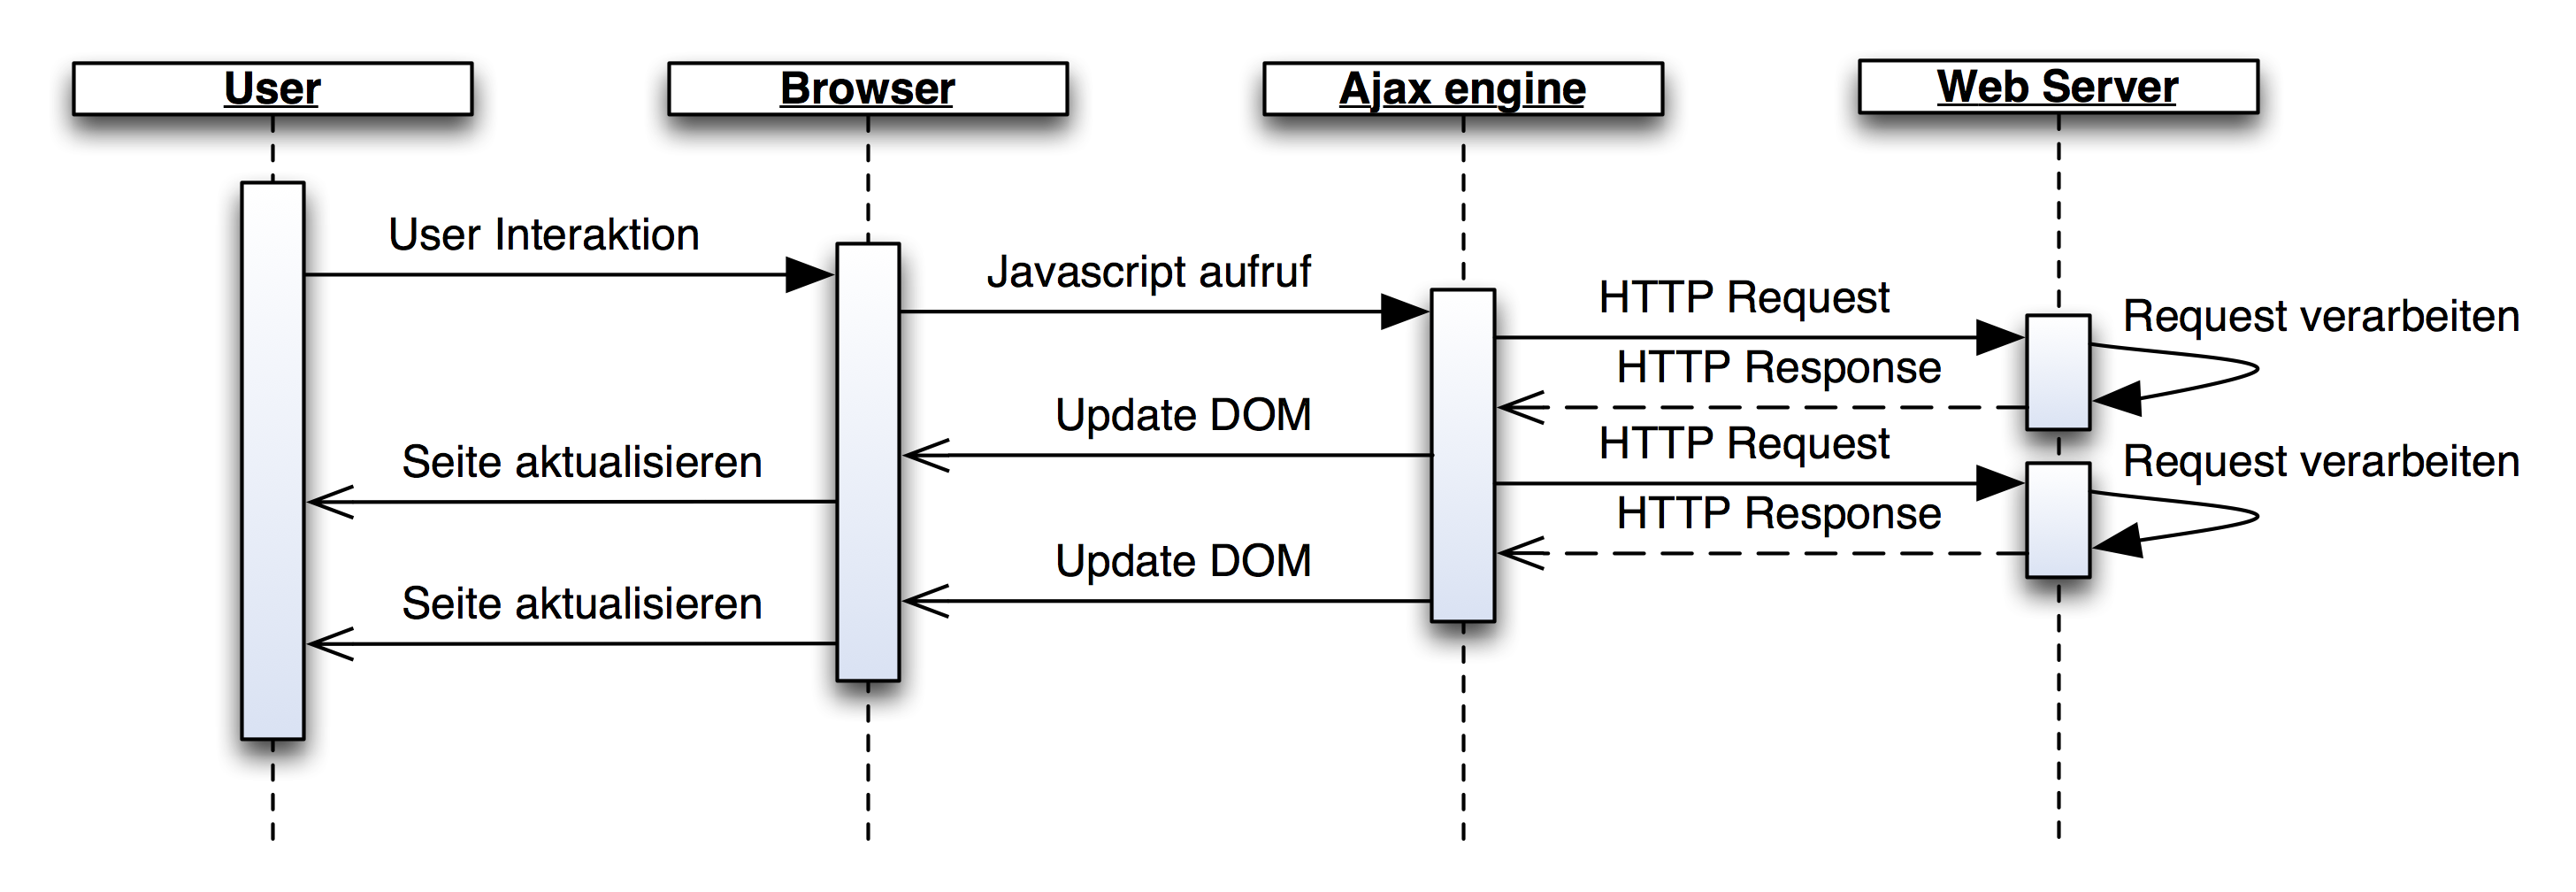
\includegraphics[width=0.85\textwidth]{./image/sequenzdiagrammAjaxPageReload.png}
      \caption{Ajax Request als \ac{UML} Sequenzdiagramm}
      \label{img:sequenzdiagrammAjaxPageReload}
    \end{center}
  \end{figure}  
  
  \subsection{Plugin orientiert}

  \subsection{Client orientiert}
  
  \section{Technologien}
  
  \subsection{Eingesetzte Standards}
  
  \subsection{Programmiermodell}
  
  \section{Security}
  
  \section{Merkmale}
    
  \subsection{Suchmaschinenoptimierung}
  
  \subsection{Barrierefreiheit}